\PassOptionsToPackage{unicode=true}{hyperref} % options for packages loaded elsewhere
\PassOptionsToPackage{hyphens}{url}
%
\documentclass[
  ignorenonframetext,
]{beamer}
\usepackage{pgfpages}
\setbeamertemplate{caption}[numbered]
\setbeamertemplate{caption label separator}{: }
\setbeamercolor{caption name}{fg=normal text.fg}
\beamertemplatenavigationsymbolsempty
% Prevent slide breaks in the middle of a paragraph:
\widowpenalties 1 10000
\raggedbottom
\setbeamertemplate{part page}{
  \centering
  \begin{beamercolorbox}[sep=16pt,center]{part title}
    \usebeamerfont{part title}\insertpart\par
  \end{beamercolorbox}
}
\setbeamertemplate{section page}{
  \centering
  \begin{beamercolorbox}[sep=12pt,center]{part title}
    \usebeamerfont{section title}\insertsection\par
  \end{beamercolorbox}
}
\setbeamertemplate{subsection page}{
  \centering
  \begin{beamercolorbox}[sep=8pt,center]{part title}
    \usebeamerfont{subsection title}\insertsubsection\par
  \end{beamercolorbox}
}
\AtBeginPart{
  \frame{\partpage}
}
\AtBeginSection{
  \ifbibliography
  \else
    \frame{\sectionpage}
  \fi
}
\AtBeginSubsection{
  \frame{\subsectionpage}
}
\usepackage{lmodern}
\usepackage{amssymb,amsmath}
\usepackage{ifxetex,ifluatex}
\ifnum 0\ifxetex 1\fi\ifluatex 1\fi=0 % if pdftex
  \usepackage[T1]{fontenc}
  \usepackage[utf8]{inputenc}
  \usepackage{textcomp} % provides euro and other symbols
\else % if luatex or xelatex
  \usepackage{unicode-math}
  \defaultfontfeatures{Scale=MatchLowercase}
  \defaultfontfeatures[\rmfamily]{Ligatures=TeX,Scale=1}
\fi
% use upquote if available, for straight quotes in verbatim environments
\IfFileExists{upquote.sty}{\usepackage{upquote}}{}
\IfFileExists{microtype.sty}{% use microtype if available
  \usepackage[]{microtype}
  \UseMicrotypeSet[protrusion]{basicmath} % disable protrusion for tt fonts
}{}
\makeatletter
\@ifundefined{KOMAClassName}{% if non-KOMA class
  \IfFileExists{parskip.sty}{%
    \usepackage{parskip}
  }{% else
    \setlength{\parindent}{0pt}
    \setlength{\parskip}{6pt plus 2pt minus 1pt}}
}{% if KOMA class
  \KOMAoptions{parskip=half}}
\makeatother
\usepackage{xcolor}
\IfFileExists{xurl.sty}{\usepackage{xurl}}{} % add URL line breaks if available
\IfFileExists{bookmark.sty}{\usepackage{bookmark}}{\usepackage{hyperref}}
\hypersetup{
  pdftitle={DSCI 415: Unsupervised Learning Final Project},
  pdfauthor={Brad Erickson \& Will Henschell},
  pdfborder={0 0 0},
  breaklinks=true}
\urlstyle{same}  % don't use monospace font for urls
\newif\ifbibliography
\usepackage{color}
\usepackage{fancyvrb}
\newcommand{\VerbBar}{|}
\newcommand{\VERB}{\Verb[commandchars=\\\{\}]}
\DefineVerbatimEnvironment{Highlighting}{Verbatim}{commandchars=\\\{\}}
% Add ',fontsize=\small' for more characters per line
\usepackage{framed}
\definecolor{shadecolor}{RGB}{248,248,248}
\newenvironment{Shaded}{\begin{snugshade}}{\end{snugshade}}
\newcommand{\AlertTok}[1]{\textcolor[rgb]{0.94,0.16,0.16}{#1}}
\newcommand{\AnnotationTok}[1]{\textcolor[rgb]{0.56,0.35,0.01}{\textbf{\textit{#1}}}}
\newcommand{\AttributeTok}[1]{\textcolor[rgb]{0.77,0.63,0.00}{#1}}
\newcommand{\BaseNTok}[1]{\textcolor[rgb]{0.00,0.00,0.81}{#1}}
\newcommand{\BuiltInTok}[1]{#1}
\newcommand{\CharTok}[1]{\textcolor[rgb]{0.31,0.60,0.02}{#1}}
\newcommand{\CommentTok}[1]{\textcolor[rgb]{0.56,0.35,0.01}{\textit{#1}}}
\newcommand{\CommentVarTok}[1]{\textcolor[rgb]{0.56,0.35,0.01}{\textbf{\textit{#1}}}}
\newcommand{\ConstantTok}[1]{\textcolor[rgb]{0.00,0.00,0.00}{#1}}
\newcommand{\ControlFlowTok}[1]{\textcolor[rgb]{0.13,0.29,0.53}{\textbf{#1}}}
\newcommand{\DataTypeTok}[1]{\textcolor[rgb]{0.13,0.29,0.53}{#1}}
\newcommand{\DecValTok}[1]{\textcolor[rgb]{0.00,0.00,0.81}{#1}}
\newcommand{\DocumentationTok}[1]{\textcolor[rgb]{0.56,0.35,0.01}{\textbf{\textit{#1}}}}
\newcommand{\ErrorTok}[1]{\textcolor[rgb]{0.64,0.00,0.00}{\textbf{#1}}}
\newcommand{\ExtensionTok}[1]{#1}
\newcommand{\FloatTok}[1]{\textcolor[rgb]{0.00,0.00,0.81}{#1}}
\newcommand{\FunctionTok}[1]{\textcolor[rgb]{0.00,0.00,0.00}{#1}}
\newcommand{\ImportTok}[1]{#1}
\newcommand{\InformationTok}[1]{\textcolor[rgb]{0.56,0.35,0.01}{\textbf{\textit{#1}}}}
\newcommand{\KeywordTok}[1]{\textcolor[rgb]{0.13,0.29,0.53}{\textbf{#1}}}
\newcommand{\NormalTok}[1]{#1}
\newcommand{\OperatorTok}[1]{\textcolor[rgb]{0.81,0.36,0.00}{\textbf{#1}}}
\newcommand{\OtherTok}[1]{\textcolor[rgb]{0.56,0.35,0.01}{#1}}
\newcommand{\PreprocessorTok}[1]{\textcolor[rgb]{0.56,0.35,0.01}{\textit{#1}}}
\newcommand{\RegionMarkerTok}[1]{#1}
\newcommand{\SpecialCharTok}[1]{\textcolor[rgb]{0.00,0.00,0.00}{#1}}
\newcommand{\SpecialStringTok}[1]{\textcolor[rgb]{0.31,0.60,0.02}{#1}}
\newcommand{\StringTok}[1]{\textcolor[rgb]{0.31,0.60,0.02}{#1}}
\newcommand{\VariableTok}[1]{\textcolor[rgb]{0.00,0.00,0.00}{#1}}
\newcommand{\VerbatimStringTok}[1]{\textcolor[rgb]{0.31,0.60,0.02}{#1}}
\newcommand{\WarningTok}[1]{\textcolor[rgb]{0.56,0.35,0.01}{\textbf{\textit{#1}}}}
\usepackage{graphicx,grffile}
\makeatletter
\def\maxwidth{\ifdim\Gin@nat@width>\linewidth\linewidth\else\Gin@nat@width\fi}
\def\maxheight{\ifdim\Gin@nat@height>\textheight\textheight\else\Gin@nat@height\fi}
\makeatother
% Scale images if necessary, so that they will not overflow the page
% margins by default, and it is still possible to overwrite the defaults
% using explicit options in \includegraphics[width, height, ...]{}
\setkeys{Gin}{width=\maxwidth,height=\maxheight,keepaspectratio}
\setlength{\emergencystretch}{3em}  % prevent overfull lines
\providecommand{\tightlist}{%
  \setlength{\itemsep}{0pt}\setlength{\parskip}{0pt}}
\setcounter{secnumdepth}{-2}

% set default figure placement to htbp
\makeatletter
\def\fps@figure{htbp}
\makeatother


\title{DSCI 415: Unsupervised Learning Final Project}
\author{Brad Erickson \& Will Henschell}
\date{}

\begin{document}
\frame{\titlepage}

\hypertarget{anime-recommender-system}{%
\section{Anime Recommender System}\label{anime-recommender-system}}

\begin{frame}[fragile]{DATA}
\protect\hypertarget{data}{}

\begin{Shaded}
\begin{Highlighting}[]
\CommentTok{#Load data (Change filepath to Anime.RData location)}
\KeywordTok{load}\NormalTok{(}\DataTypeTok{file=}\StringTok{"C:/Users/ic2009ml/Documents/GitHub/DSCI415-Final-Project/data/Anime.RData"}\NormalTok{)}
\KeywordTok{colnames}\NormalTok{(tv[}\DecValTok{1}\OperatorTok{:}\DecValTok{10}\NormalTok{])}
\end{Highlighting}
\end{Shaded}

\begin{verbatim}
##  [1] ".hack..Roots"                                 
##  [2] ".hack..Sign"                                  
##  [3] ".hack..Tasogare.no.Udewa.Densetsu"            
##  [4] "X009.1"                                       
##  [5] "X07.Ghost"                                    
##  [6] "X11eyes"                                      
##  [7] "X12.sai...Chicchana.Mune.no.Tokimeki"         
##  [8] "X3.Choume.no.Tama..Uchi.no.Tama.Shirimasenka."
##  [9] "X30.sai.no.Hoken.Taiiku"                      
## [10] "X91.Days"
\end{verbatim}

\end{frame}

\begin{frame}[fragile]{MODEL SELECTION EVALUATION}
\protect\hypertarget{model-selection-evaluation}{}

\begin{Shaded}
\begin{Highlighting}[]
\CommentTok{#Testing all recommenders}
\NormalTok{explore.scheme =}\StringTok{ }\KeywordTok{evaluationScheme}\NormalTok{(tv.mat, }\DataTypeTok{method=} \StringTok{'split'}\NormalTok{, }\DataTypeTok{train =} \FloatTok{0.85}\NormalTok{, }\DataTypeTok{k =} \DecValTok{1}\NormalTok{, }\DataTypeTok{given =} \DecValTok{1}\NormalTok{, }\DataTypeTok{goodRating =} \DecValTok{7}\NormalTok{)}

\CommentTok{#Setting algorithms to test}
\NormalTok{explore.algorithms <-}\StringTok{ }\KeywordTok{list}\NormalTok{(}
  \StringTok{'random items'}\NormalTok{ =}\StringTok{ }\KeywordTok{list}\NormalTok{(}\DataTypeTok{name =} \StringTok{'RANDOM'}\NormalTok{, }\DataTypeTok{param =} \KeywordTok{list}\NormalTok{(}\DataTypeTok{normalize =} \StringTok{'Z-score'}\NormalTok{)),}
  \StringTok{'popular items'}\NormalTok{ =}\StringTok{ }\KeywordTok{list}\NormalTok{(}\DataTypeTok{name =} \StringTok{'POPULAR'}\NormalTok{, }\DataTypeTok{param =} \KeywordTok{list}\NormalTok{(}\DataTypeTok{normalize =} \StringTok{'Z-score'}\NormalTok{)),}
  \StringTok{'user-based CF'}\NormalTok{ =}\StringTok{ }\KeywordTok{list}\NormalTok{(}\DataTypeTok{name =} \StringTok{'UBCF'}\NormalTok{, }\DataTypeTok{param =} \KeywordTok{list}\NormalTok{(}\DataTypeTok{normalize =} \StringTok{'Z-score'}\NormalTok{, }\DataTypeTok{method =} \StringTok{'Cosine'}\NormalTok{, }\DataTypeTok{nn=}\DecValTok{50}\NormalTok{)),}
  \StringTok{'item-based CF'}\NormalTok{ =}\StringTok{ }\KeywordTok{list}\NormalTok{(}\DataTypeTok{name =} \StringTok{'IBCF'}\NormalTok{, }\DataTypeTok{param =} \KeywordTok{list}\NormalTok{(}\DataTypeTok{normalize =} \StringTok{'Z-score'}\NormalTok{))}
\NormalTok{  )}

\CommentTok{#Evaluating all algorithms}
\NormalTok{explore.results =}\StringTok{ }\KeywordTok{evaluate}\NormalTok{(explore.scheme, explore.algorithms, }\DataTypeTok{n=}\KeywordTok{c}\NormalTok{(}\DecValTok{1}\NormalTok{, }\DecValTok{3}\NormalTok{, }\DecValTok{5}\NormalTok{, }\DecValTok{10}\NormalTok{, }\DecValTok{15}\NormalTok{, }\DecValTok{20}\NormalTok{))}
\end{Highlighting}
\end{Shaded}

\end{frame}

\begin{frame}[fragile]{Plotting model results for comparison (TPR and
FPR)}
\protect\hypertarget{plotting-model-results-for-comparison-tpr-and-fpr}{}

\begin{Shaded}
\begin{Highlighting}[]
\KeywordTok{plot}\NormalTok{(explore.results, }\DataTypeTok{annotate =} \DecValTok{1}\OperatorTok{:}\DecValTok{4}\NormalTok{, }\DataTypeTok{legend =} \StringTok{'topleft'}\NormalTok{)}
\end{Highlighting}
\end{Shaded}

\includegraphics{final_presentation_files/figure-beamer/anime.plotting.TPR.and.FPR.model-1.pdf}

\end{frame}

\begin{frame}[fragile]{Plotting model results for comparison (precision
and recall)}
\protect\hypertarget{plotting-model-results-for-comparison-precision-and-recall}{}

\begin{Shaded}
\begin{Highlighting}[]
\KeywordTok{plot}\NormalTok{(explore.results, }\StringTok{'prec/rec'}\NormalTok{, }\DataTypeTok{annotate =} \DecValTok{2}\OperatorTok{:}\DecValTok{3}\NormalTok{)}
\end{Highlighting}
\end{Shaded}

\includegraphics{final_presentation_files/figure-beamer/anime.plotting.precision.and.recall.model-1.pdf}

\end{frame}

\begin{frame}[fragile]{FINAL RECOMMENDER MODEL}
\protect\hypertarget{final-recommender-model}{}

\begin{Shaded}
\begin{Highlighting}[]
\CommentTok{#Creating test and training data for final model}
\NormalTok{tv.scheme =}\StringTok{ }\KeywordTok{evaluationScheme}\NormalTok{(tv.mat, }\DataTypeTok{method=} \StringTok{'split'}\NormalTok{, }\DataTypeTok{train =} \FloatTok{0.666666}\NormalTok{, }\DataTypeTok{given =} \DecValTok{1}\NormalTok{, }\DataTypeTok{goodRating =} \DecValTok{7}\NormalTok{)}

\CommentTok{#Fitting the popular items recommender on the training data}
\NormalTok{tv.pop.rec =}\StringTok{ }\KeywordTok{Recommender}\NormalTok{(}\KeywordTok{getData}\NormalTok{(tv.scheme, }\StringTok{'train'}\NormalTok{), }\DataTypeTok{method =} \StringTok{'POPULAR'}\NormalTok{)}
\end{Highlighting}
\end{Shaded}

\end{frame}

\begin{frame}[fragile]{Creating top 10 list for all users}
\protect\hypertarget{creating-top-10-list-for-all-users}{}

\begin{Shaded}
\begin{Highlighting}[]
\NormalTok{new.users.top10 =}\StringTok{ }\KeywordTok{predict}\NormalTok{(tv.pop.rec, }\KeywordTok{getData}\NormalTok{(tv.scheme, }\StringTok{'known'}\NormalTok{), }\DataTypeTok{n=}\DecValTok{10}\NormalTok{)}
\KeywordTok{as}\NormalTok{(new.users.top10, }\StringTok{'list'}\NormalTok{)}
\end{Highlighting}
\end{Shaded}

\end{frame}

\begin{frame}[fragile]{Creating top 10 list for sample of 10}
\protect\hypertarget{creating-top-10-list-for-sample-of-10}{}

\begin{Shaded}
\begin{Highlighting}[]
\NormalTok{sample.new.users.top10 =}\StringTok{ }\KeywordTok{predict}\NormalTok{(tv.pop.rec, }\KeywordTok{getData}\NormalTok{(tv.scheme, }\StringTok{'known'}\NormalTok{)[}\DecValTok{1}\OperatorTok{:}\DecValTok{10}\NormalTok{,], }\DataTypeTok{n=}\DecValTok{10}\NormalTok{)}
\NormalTok{sample.new.users.top10.list <-}\StringTok{ }\KeywordTok{as}\NormalTok{(sample.new.users.top10, }\StringTok{'list'}\NormalTok{)}
\end{Highlighting}
\end{Shaded}

\end{frame}

\begin{frame}[fragile]{Printing top 10 list for sample of 10}
\protect\hypertarget{printing-top-10-list-for-sample-of-10}{}

\begin{Shaded}
\begin{Highlighting}[]
\NormalTok{sample.new.users.top10.list}
\end{Highlighting}
\end{Shaded}

\begin{verbatim}
## [[1]]
##  [1] "Fullmetal.Alchemist..Brotherhood"   "Death.Note"                        
##  [3] "Steins.Gate"                        "Code.Geass..Hangyaku.no.Lelouch.R2"
##  [5] "Code.Geass..Hangyaku.no.Lelouch"    "Clannad..After.Story"              
##  [7] "Tengen.Toppa.Gurren.Lagann"         "Shingeki.no.Kyojin"                
##  [9] "Cowboy.Bebop"                       "Toradora."                         
## 
## [[2]]
##  [1] "Fullmetal.Alchemist..Brotherhood"   "Death.Note"                        
##  [3] "Steins.Gate"                        "Code.Geass..Hangyaku.no.Lelouch.R2"
##  [5] "Code.Geass..Hangyaku.no.Lelouch"    "Clannad..After.Story"              
##  [7] "Tengen.Toppa.Gurren.Lagann"         "Shingeki.no.Kyojin"                
##  [9] "Cowboy.Bebop"                       "Toradora."                         
## 
## [[3]]
##  [1] "Fullmetal.Alchemist..Brotherhood"   "Death.Note"                        
##  [3] "Steins.Gate"                        "Code.Geass..Hangyaku.no.Lelouch.R2"
##  [5] "Clannad..After.Story"               "Tengen.Toppa.Gurren.Lagann"        
##  [7] "Shingeki.no.Kyojin"                 "Cowboy.Bebop"                      
##  [9] "Toradora."                          "Angel.Beats."                      
## 
## [[4]]
##  [1] "Fullmetal.Alchemist..Brotherhood"   "Death.Note"                        
##  [3] "Steins.Gate"                        "Code.Geass..Hangyaku.no.Lelouch.R2"
##  [5] "Code.Geass..Hangyaku.no.Lelouch"    "Clannad..After.Story"              
##  [7] "Tengen.Toppa.Gurren.Lagann"         "Shingeki.no.Kyojin"                
##  [9] "Cowboy.Bebop"                       "Toradora."                         
## 
## [[5]]
##  [1] "Fullmetal.Alchemist..Brotherhood"   "Death.Note"                        
##  [3] "Steins.Gate"                        "Code.Geass..Hangyaku.no.Lelouch.R2"
##  [5] "Code.Geass..Hangyaku.no.Lelouch"    "Clannad..After.Story"              
##  [7] "Tengen.Toppa.Gurren.Lagann"         "Cowboy.Bebop"                      
##  [9] "Toradora."                          "Angel.Beats."                      
## 
## [[6]]
##  [1] "Fullmetal.Alchemist..Brotherhood"   "Death.Note"                        
##  [3] "Steins.Gate"                        "Code.Geass..Hangyaku.no.Lelouch.R2"
##  [5] "Code.Geass..Hangyaku.no.Lelouch"    "Clannad..After.Story"              
##  [7] "Tengen.Toppa.Gurren.Lagann"         "Shingeki.no.Kyojin"                
##  [9] "Cowboy.Bebop"                       "Toradora."                         
## 
## [[7]]
##  [1] "Fullmetal.Alchemist..Brotherhood"   "Death.Note"                        
##  [3] "Steins.Gate"                        "Code.Geass..Hangyaku.no.Lelouch.R2"
##  [5] "Code.Geass..Hangyaku.no.Lelouch"    "Clannad..After.Story"              
##  [7] "Tengen.Toppa.Gurren.Lagann"         "Shingeki.no.Kyojin"                
##  [9] "Cowboy.Bebop"                       "Toradora."                         
## 
## [[8]]
##  [1] "Fullmetal.Alchemist..Brotherhood"   "Death.Note"                        
##  [3] "Steins.Gate"                        "Code.Geass..Hangyaku.no.Lelouch.R2"
##  [5] "Code.Geass..Hangyaku.no.Lelouch"    "Clannad..After.Story"              
##  [7] "Tengen.Toppa.Gurren.Lagann"         "Shingeki.no.Kyojin"                
##  [9] "Cowboy.Bebop"                       "Toradora."                         
## 
## [[9]]
##  [1] "Fullmetal.Alchemist..Brotherhood"   "Death.Note"                        
##  [3] "Steins.Gate"                        "Code.Geass..Hangyaku.no.Lelouch.R2"
##  [5] "Code.Geass..Hangyaku.no.Lelouch"    "Clannad..After.Story"              
##  [7] "Tengen.Toppa.Gurren.Lagann"         "Shingeki.no.Kyojin"                
##  [9] "Cowboy.Bebop"                       "Toradora."                         
## 
## [[10]]
##  [1] "Fullmetal.Alchemist..Brotherhood"   "Steins.Gate"                       
##  [3] "Code.Geass..Hangyaku.no.Lelouch.R2" "Code.Geass..Hangyaku.no.Lelouch"   
##  [5] "Clannad..After.Story"               "Tengen.Toppa.Gurren.Lagann"        
##  [7] "Shingeki.no.Kyojin"                 "Cowboy.Bebop"                      
##  [9] "Toradora."                          "Angel.Beats."
\end{verbatim}

\end{frame}

\begin{frame}[fragile]{Creating and cleaning a string version of the
list for the sample of 10}
\protect\hypertarget{creating-and-cleaning-a-string-version-of-the-list-for-the-sample-of-10}{}

\begin{Shaded}
\begin{Highlighting}[]
\NormalTok{sample.new.users.top10.string <-}\StringTok{ }\KeywordTok{as.character}\NormalTok{(sample.new.users.top10.list)}
\NormalTok{sample.new.users.top10.string <-}\StringTok{ }\KeywordTok{gsub}\NormalTok{(}\StringTok{'c}\CharTok{\textbackslash{}\textbackslash{}}\StringTok{('}\NormalTok{, }\StringTok{''}\NormalTok{, sample.new.users.top10.string)}
\NormalTok{sample.new.users.top10.string <-}\StringTok{ }\KeywordTok{gsub}\NormalTok{(}\StringTok{'}\CharTok{\textbackslash{}\textbackslash{}}\StringTok{)'}\NormalTok{, }\StringTok{''}\NormalTok{, sample.new.users.top10.string)}
\end{Highlighting}
\end{Shaded}

\end{frame}

\begin{frame}[fragile]{Preparing the counts of anime TV series that
appear in the top 10 list for 10 users}
\protect\hypertarget{preparing-the-counts-of-anime-tv-series-that-appear-in-the-top-10-list-for-10-users}{}

\begin{Shaded}
\begin{Highlighting}[]
\NormalTok{sample.new.users.top10.list.split <-}\StringTok{ }\KeywordTok{unlist}\NormalTok{(}\KeywordTok{strsplit}\NormalTok{(sample.new.users.top10.string, }\DataTypeTok{split =} \StringTok{','}\NormalTok{))}
\NormalTok{sample.new.users.top10.list.split.dt <-}\StringTok{ }\KeywordTok{data.table}\NormalTok{(sample.new.users.top10.list.split)}
\KeywordTok{colnames}\NormalTok{(sample.new.users.top10.list.split.dt)[}\KeywordTok{colnames}\NormalTok{(sample.new.users.top10.list.split.dt)}\OperatorTok{==}\StringTok{"sample.new.users.top10.list.split"}\NormalTok{] <-}\StringTok{ "anime_title"}
\NormalTok{sample.new.users.top10.anime.counts <-}\StringTok{ }\NormalTok{sample.new.users.top10.list.split.dt[, .(}\DataTypeTok{count =}\NormalTok{ .N), by =}\StringTok{ }\NormalTok{sample.new.users.top10.list.split.dt[,}\DecValTok{1}\NormalTok{]]}
\end{Highlighting}
\end{Shaded}

\end{frame}

\begin{frame}[fragile]{Printing top anime counts for sample of 10 users}
\protect\hypertarget{printing-top-anime-counts-for-sample-of-10-users}{}

\begin{Shaded}
\begin{Highlighting}[]
\KeywordTok{print}\NormalTok{(sample.new.users.top10.anime.counts)}
\end{Highlighting}
\end{Shaded}

\begin{verbatim}
##                               anime_title count
##  1:    "Fullmetal.Alchemist..Brotherhood"    10
##  2:                          "Death.Note"     9
##  3:                         "Steins.Gate"    10
##  4:  "Code.Geass..Hangyaku.no.Lelouch.R2"    10
##  5:     "Code.Geass..Hangyaku.no.Lelouch"     9
##  6:                "Clannad..After.Story"    10
##  7:          "Tengen.Toppa.Gurren.Lagann"    10
##  8:                  "Shingeki.no.Kyojin"     9
##  9:                        "Cowboy.Bebop"    10
## 10:                           "Toradora."    10
## 11:                        "Angel.Beats."     3
\end{verbatim}

\end{frame}

\hypertarget{pokemon-cluster-analysis}{%
\section{Pokemon Cluster Analysis}\label{pokemon-cluster-analysis}}

\begin{frame}[fragile]{Overall data}
\protect\hypertarget{overall-data}{}

\begin{Shaded}
\begin{Highlighting}[]
\KeywordTok{colnames}\NormalTok{(pokemon)}
\end{Highlighting}
\end{Shaded}

\begin{verbatim}
##  [1] "abilities"         "against_bug"       "against_dark"     
##  [4] "against_dragon"    "against_electric"  "against_fairy"    
##  [7] "against_fight"     "against_fire"      "against_flying"   
## [10] "against_ghost"     "against_grass"     "against_ground"   
## [13] "against_ice"       "against_normal"    "against_poison"   
## [16] "against_psychic"   "against_rock"      "against_steel"    
## [19] "against_water"     "attack"            "base_egg_steps"   
## [22] "base_happiness"    "base_total"        "capture_rate"     
## [25] "classfication"     "defense"           "experience_growth"
## [28] "height_m"          "hp"                "japanese_name"    
## [31] "name"              "percentage_male"   "pokedex_number"   
## [34] "sp_attack"         "sp_defense"        "speed"            
## [37] "type1"             "type2"             "weight_kg"        
## [40] "generation"        "is_legendary"      "type"             
## [43] "name.type"
\end{verbatim}

\end{frame}

\begin{frame}[fragile]{Data for clustering}
\protect\hypertarget{data-for-clustering}{}

\begin{Shaded}
\begin{Highlighting}[]
\KeywordTok{colnames}\NormalTok{(pokemon[}\DecValTok{2}\OperatorTok{:}\DecValTok{19}\NormalTok{])}
\end{Highlighting}
\end{Shaded}

\begin{verbatim}
##  [1] "against_bug"      "against_dark"     "against_dragon"   "against_electric"
##  [5] "against_fairy"    "against_fight"    "against_fire"     "against_flying"  
##  [9] "against_ghost"    "against_grass"    "against_ground"   "against_ice"     
## [13] "against_normal"   "against_poison"   "against_psychic"  "against_rock"    
## [17] "against_steel"    "against_water"
\end{verbatim}

\begin{Shaded}
\begin{Highlighting}[]
\NormalTok{pokemon.mat[}\DecValTok{1}\NormalTok{,]}
\end{Highlighting}
\end{Shaded}

\begin{verbatim}
##                        against_bug against_dark against_dragon against_electric
## grass poison Bulbasaur           1            1              1              0.5
##                        against_fairy against_fight against_fire against_flying
## grass poison Bulbasaur           0.5           0.5            2              2
##                        against_ghost against_grass against_ground against_ice
## grass poison Bulbasaur             1          0.25              1           2
##                        against_normal against_poison against_psychic
## grass poison Bulbasaur              1              1               2
##                        against_rock against_steel against_water
## grass poison Bulbasaur            1             1           0.5
\end{verbatim}

\end{frame}

\begin{frame}[fragile]{Finding k: wss}
\protect\hypertarget{finding-k-wss}{}

\begin{Shaded}
\begin{Highlighting}[]
\KeywordTok{fviz_nbclust}\NormalTok{(pokemon.mat,kmeans,}\DataTypeTok{k.max=}\DecValTok{25}\NormalTok{,}\DataTypeTok{method=}\StringTok{"wss"}\NormalTok{)}
\end{Highlighting}
\end{Shaded}

\includegraphics{final_presentation_files/figure-beamer/pokemon.finding.k.wss-1.pdf}

\end{frame}

\begin{frame}[fragile]{Finding k: silhouette}
\protect\hypertarget{finding-k-silhouette}{}

\begin{Shaded}
\begin{Highlighting}[]
\KeywordTok{fviz_nbclust}\NormalTok{(pokemon.mat,kmeans,}\DataTypeTok{k.max=}\DecValTok{25}\NormalTok{,}\DataTypeTok{method=}\StringTok{"silhouette"}\NormalTok{)}
\end{Highlighting}
\end{Shaded}

\includegraphics{final_presentation_files/figure-beamer/pokemon.finding.k.silhouette-1.pdf}

\end{frame}

\begin{frame}[fragile]{Finding k: gap\_stat}
\protect\hypertarget{finding-k-gap_stat}{}

\begin{Shaded}
\begin{Highlighting}[]
\KeywordTok{fviz_nbclust}\NormalTok{(pokemon.mat,kmeans,}\DataTypeTok{k.max=}\DecValTok{25}\NormalTok{,}\DataTypeTok{method=}\StringTok{"gap_stat"}\NormalTok{)}
\end{Highlighting}
\end{Shaded}

\includegraphics{final_presentation_files/figure-beamer/pokemon.finding.k.gap_stat-1.pdf}

\end{frame}

\begin{frame}{Hierarchical clustering}
\protect\hypertarget{hierarchical-clustering}{}

We choose k = 18 which is the total number of types
\includegraphics{final_presentation_files/figure-beamer/pokemon.hclust-1.pdf}

\end{frame}

\begin{frame}{Zoomed on clusters 1}
\protect\hypertarget{zoomed-on-clusters-1}{}

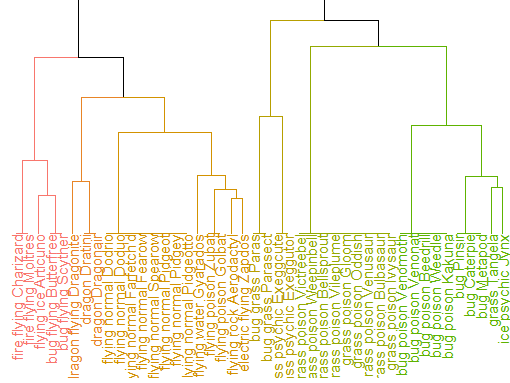
\includegraphics{pokemon_dend_01.PNG}

\end{frame}

\begin{frame}{Zoomed on clusters 2}
\protect\hypertarget{zoomed-on-clusters-2}{}

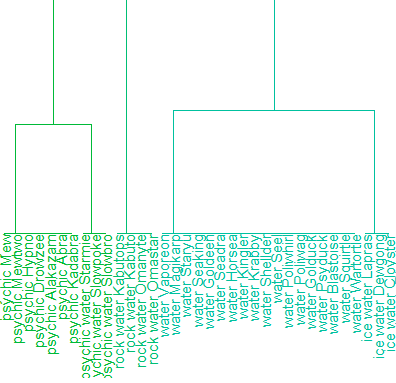
\includegraphics{pokemon_dend_02.PNG}

\end{frame}

\begin{frame}{Zoomed on clusters 3}
\protect\hypertarget{zoomed-on-clusters-3}{}

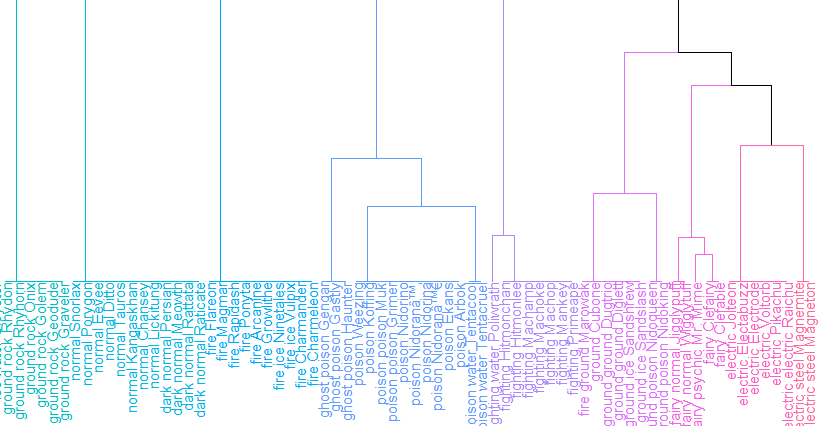
\includegraphics{pokemon_dend_03.PNG}

\end{frame}

\hypertarget{seinfeld-text-mining}{%
\section{Seinfeld Text Mining}\label{seinfeld-text-mining}}

\begin{frame}[fragile]{Data}
\protect\hypertarget{data-1}{}

\begin{Shaded}
\begin{Highlighting}[]
\KeywordTok{colnames}\NormalTok{(show)}
\end{Highlighting}
\end{Shaded}

\begin{verbatim}
## [1] "X"         "Character" "Dialogue"  "EpisodeNo" "SEID"      "Season"
\end{verbatim}

\end{frame}

\begin{frame}[fragile]{Sentiment analysis per season}
\protect\hypertarget{sentiment-analysis-per-season}{}

\begin{Shaded}
\begin{Highlighting}[]
\ControlFlowTok{for}\NormalTok{ (i }\ControlFlowTok{in}\NormalTok{ seasons) \{}
\NormalTok{  season.data <-}\StringTok{ }\NormalTok{show }\OperatorTok\StringTok{ }\KeywordTok{filter}\NormalTok{(Season}\OperatorTok{==}\NormalTok{i)}
\NormalTok{  episodes <-}\StringTok{ }\KeywordTok{unique}\NormalTok{(season.data}\OperatorTok{$}\NormalTok{EpisodeNo)}
\NormalTok{  season.sentiment <-}\StringTok{ }\KeywordTok{data.frame}\NormalTok{()}
\NormalTok{  title <-}\StringTok{ }\KeywordTok{paste}\NormalTok{(show.title,}\StringTok{": Season "}\NormalTok{,i,}\StringTok{" sentiment by episode"}\NormalTok{)}
  \KeywordTok{plot}\NormalTok{(}\DecValTok{0}\NormalTok{,}\DecValTok{0}\NormalTok{, }\DataTypeTok{main=}\NormalTok{title, }\DataTypeTok{xlab =} \StringTok{"Normalized Narrative Time"}\NormalTok{, }\DataTypeTok{ylab =} \StringTok{"Scaled Sentiment"}\NormalTok{, }\DataTypeTok{type=}\StringTok{"n"}\NormalTok{, }\DataTypeTok{xlim=}\KeywordTok{c}\NormalTok{(}\OperatorTok{-}\DecValTok{1}\NormalTok{,}\DecValTok{101}\NormalTok{), }\DataTypeTok{ylim=}\KeywordTok{c}\NormalTok{(}\OperatorTok{-}\FloatTok{1.01}\NormalTok{, }\FloatTok{1.01}\NormalTok{))}
  \ControlFlowTok{for}\NormalTok{ (j }\ControlFlowTok{in}\NormalTok{ episodes) \{}
\NormalTok{    episode.data <-}\StringTok{ }\NormalTok{season.data }\OperatorTok\StringTok{ }\KeywordTok{filter}\NormalTok{(EpisodeNo}\OperatorTok{==}\NormalTok{j)}
\NormalTok{    episode.sentences <-}\StringTok{ }\KeywordTok{get_sentences}\NormalTok{(episode.data}\OperatorTok{$}\NormalTok{Dialogue)}
\NormalTok{    episode.sentiment <-}\StringTok{ }\KeywordTok{get_sentiment}\NormalTok{(episode.sentences)}
\NormalTok{    episode.sentiment.values <-}\StringTok{ }\KeywordTok{get_dct_transform}\NormalTok{(episode.sentiment, }\DataTypeTok{low_pass_size =} \DecValTok{5}\NormalTok{, }\DataTypeTok{x_reverse_len =} \DecValTok{100}\NormalTok{, }\DataTypeTok{scale_vals =}\NormalTok{ F, }\DataTypeTok{scale_range =}\NormalTok{ T)}
\NormalTok{    season.sentiment <-}\StringTok{ }\KeywordTok{cbind.all}\NormalTok{(season.sentiment, episode.sentiment.values)}
    \KeywordTok{lines}\NormalTok{(episode.sentiment.values)}
\NormalTok{  \}}
\NormalTok{  season.sentiment.means <-}\StringTok{ }\KeywordTok{rowMeans}\NormalTok{(season.sentiment)}
  \KeywordTok{lines}\NormalTok{(season.sentiment.means, }\DataTypeTok{col=}\StringTok{"firebrick"}\NormalTok{, }\DataTypeTok{lwd =} \DecValTok{5}\NormalTok{)}
\NormalTok{\}}
\end{Highlighting}
\end{Shaded}

\end{frame}

\begin{frame}{Seinfeld : Season 1 sentiment by
episode\includegraphics{final_presentation_files/figure-beamer/unnamed-chunk-2-1.pdf}}
\protect\hypertarget{seinfeld-season-1-sentiment-by-episode}{}

\end{frame}

\begin{frame}{Seinfeld : Season 2 sentiment by
episode\includegraphics{final_presentation_files/figure-beamer/unnamed-chunk-2-2.pdf}}
\protect\hypertarget{seinfeld-season-2-sentiment-by-episode}{}

\end{frame}

\begin{frame}{Seinfeld : Season 3 sentiment by
episode\includegraphics{final_presentation_files/figure-beamer/unnamed-chunk-2-3.pdf}}
\protect\hypertarget{seinfeld-season-3-sentiment-by-episode}{}

\end{frame}

\begin{frame}{Seinfeld : Season 4 sentiment by
episode\includegraphics{final_presentation_files/figure-beamer/unnamed-chunk-2-4.pdf}}
\protect\hypertarget{seinfeld-season-4-sentiment-by-episode}{}

\end{frame}

\begin{frame}{Seinfeld : Season 5 sentiment by
episode\includegraphics{final_presentation_files/figure-beamer/unnamed-chunk-2-5.pdf}}
\protect\hypertarget{seinfeld-season-5-sentiment-by-episode}{}

\end{frame}

\begin{frame}{Seinfeld : Season 6 sentiment by
episode\includegraphics{final_presentation_files/figure-beamer/unnamed-chunk-2-6.pdf}}
\protect\hypertarget{seinfeld-season-6-sentiment-by-episode}{}

\end{frame}

\begin{frame}{Seinfeld : Season 7 sentiment by
episode\includegraphics{final_presentation_files/figure-beamer/unnamed-chunk-2-7.pdf}}
\protect\hypertarget{seinfeld-season-7-sentiment-by-episode}{}

\end{frame}

\begin{frame}{Seinfeld : Season 8 sentiment by
episode\includegraphics{final_presentation_files/figure-beamer/unnamed-chunk-2-8.pdf}}
\protect\hypertarget{seinfeld-season-8-sentiment-by-episode}{}

\end{frame}

\begin{frame}{Seinfeld : Season 9 sentiment by
episode\includegraphics{final_presentation_files/figure-beamer/unnamed-chunk-2-9.pdf}}
\protect\hypertarget{seinfeld-season-9-sentiment-by-episode}{}

\end{frame}

\begin{frame}[fragile]{Sentiment analysis overall}
\protect\hypertarget{sentiment-analysis-overall}{}

\begin{Shaded}
\begin{Highlighting}[]
\NormalTok{title <-}\StringTok{ }\KeywordTok{paste}\NormalTok{(show.title,}\StringTok{": Sentiment by season"}\NormalTok{)}
\KeywordTok{plot}\NormalTok{(}\DecValTok{0}\NormalTok{,}\DecValTok{0}\NormalTok{, }\DataTypeTok{main=}\NormalTok{title, }\DataTypeTok{xlab =} \StringTok{"Normalized Narrative Time"}\NormalTok{, }\DataTypeTok{ylab =} \StringTok{"Scaled Sentiment"}\NormalTok{, }\DataTypeTok{type=}\StringTok{"n"}\NormalTok{, }\DataTypeTok{xlim=}\KeywordTok{c}\NormalTok{(}\OperatorTok{-}\DecValTok{1}\NormalTok{,}\DecValTok{101}\NormalTok{), }\DataTypeTok{ylim=}\KeywordTok{c}\NormalTok{(}\OperatorTok{-}\FloatTok{1.01}\NormalTok{, }\FloatTok{1.01}\NormalTok{))}
\ControlFlowTok{for}\NormalTok{ (i }\ControlFlowTok{in}\NormalTok{ seasons) \{}
  \KeywordTok{lines}\NormalTok{(show.sentiment[,i], }\DataTypeTok{col=}\NormalTok{i)}
\NormalTok{\}}
\KeywordTok{lines}\NormalTok{(}\KeywordTok{rowMeans}\NormalTok{(episodes.sentiment), }\DataTypeTok{col=}\StringTok{"firebrick"}\NormalTok{, }\DataTypeTok{lwd =} \DecValTok{5}\NormalTok{)}
\end{Highlighting}
\end{Shaded}

\end{frame}

\begin{frame}{Seinfeld : Sentiment by
season\includegraphics{final_presentation_files/figure-beamer/unnamed-chunk-3-1.pdf}}
\protect\hypertarget{seinfeld-sentiment-by-season}{}

\end{frame}

\begin{frame}[fragile]{Wordcloud individual code}
\protect\hypertarget{wordcloud-individual-code}{}

\begin{Shaded}
\begin{Highlighting}[]
\NormalTok{main.characters <-}\StringTok{ }\KeywordTok{c}\NormalTok{(}\StringTok{"JERRY"}\NormalTok{, }\StringTok{"GEORGE"}\NormalTok{, }\StringTok{"ELAINE"}\NormalTok{, }\StringTok{"KRAMER"}\NormalTok{)}
\ControlFlowTok{for}\NormalTok{ (i }\ControlFlowTok{in}\NormalTok{ main.characters) \{}
\NormalTok{  character.data <-}\StringTok{ }\NormalTok{show }\OperatorTok\StringTok{ }\KeywordTok{filter}\NormalTok{(}\KeywordTok{grepl}\NormalTok{(i,Character))}
\NormalTok{  character.text.clean <-}\StringTok{ }\KeywordTok{clean.text}\NormalTok{(character.data}\OperatorTok{$}\NormalTok{Dialogue)}
\NormalTok{  character.corpus.stop <-}\StringTok{ }\KeywordTok{Corpus}\NormalTok{(}\KeywordTok{VectorSource}\NormalTok{(character.text.clean))}
\NormalTok{  character.corpus <-}\StringTok{ }\KeywordTok{tm_map}\NormalTok{(character.corpus.stop, removeWords, }\KeywordTok{stopwords}\NormalTok{(}\StringTok{"en"}\NormalTok{))}
\NormalTok{  character.TDM <-}\StringTok{ }\KeywordTok{TermDocumentMatrix}\NormalTok{(character.corpus)}
\NormalTok{  character.matrix <-}\StringTok{ }\KeywordTok{as.matrix}\NormalTok{(character.TDM)}
\NormalTok{  character.freq <-}\StringTok{ }\KeywordTok{rowSums}\NormalTok{(character.matrix)}
\NormalTok{  character.freq <-}\StringTok{ }\KeywordTok{sort}\NormalTok{(character.freq, }\DataTypeTok{decreasing=}\NormalTok{T)}
  \KeywordTok{wordcloud}\NormalTok{(}\DataTypeTok{words=}\KeywordTok{names}\NormalTok{(character.freq[}\DecValTok{1}\OperatorTok{:}\DecValTok{100}\NormalTok{]), }\DataTypeTok{freq=}\NormalTok{character.freq[}\DecValTok{1}\OperatorTok{:}\DecValTok{100}\NormalTok{], }\DataTypeTok{col=}\KeywordTok{rainbow}\NormalTok{(}\DecValTok{1000}\NormalTok{))}
\NormalTok{\}}
\end{Highlighting}
\end{Shaded}

\end{frame}

\begin{frame}{Seinfeld : JERRY top 20 most used
words\includegraphics{final_presentation_files/figure-beamer/unnamed-chunk-4-1.pdf}}
\protect\hypertarget{seinfeld-jerry-top-20-most-used-words}{}

\end{frame}

\begin{frame}{Seinfeld : GEORGE top 20 most used
words\includegraphics{final_presentation_files/figure-beamer/unnamed-chunk-4-2.pdf}}
\protect\hypertarget{seinfeld-george-top-20-most-used-words}{}

\end{frame}

\begin{frame}{Seinfeld : ELAINE top 20 most used
words\includegraphics{final_presentation_files/figure-beamer/unnamed-chunk-4-3.pdf}}
\protect\hypertarget{seinfeld-elaine-top-20-most-used-words}{}

\end{frame}

\begin{frame}{Seinfeld : KRAMER top 20 most used
words\includegraphics{final_presentation_files/figure-beamer/unnamed-chunk-4-4.pdf}}
\protect\hypertarget{seinfeld-kramer-top-20-most-used-words}{}

\end{frame}

\begin{frame}[fragile]{Wordcloud comparison code}
\protect\hypertarget{wordcloud-comparison-code}{}

\begin{Shaded}
\begin{Highlighting}[]
\NormalTok{group <-}\StringTok{ }\KeywordTok{c}\NormalTok{(jerry, george, elaine, kramer)}
\NormalTok{group <-}\StringTok{ }\KeywordTok{removeWords}\NormalTok{(group, }\KeywordTok{stopwords}\NormalTok{(}\StringTok{"english"}\NormalTok{))}

\NormalTok{group.corpus <-}\StringTok{ }\KeywordTok{Corpus}\NormalTok{(}\KeywordTok{VectorSource}\NormalTok{(group))}
\NormalTok{group.TDM <-}\StringTok{ }\KeywordTok{TermDocumentMatrix}\NormalTok{(group.corpus)}
\NormalTok{group.mat <-}\StringTok{ }\KeywordTok{as.matrix}\NormalTok{(group.TDM)}
\KeywordTok{colnames}\NormalTok{(group.mat) <-}\StringTok{ }\KeywordTok{c}\NormalTok{(}\StringTok{"JERRY"}\NormalTok{, }\StringTok{"GEORGE"}\NormalTok{, }\StringTok{"ELAINE"}\NormalTok{, }\StringTok{"KRAMER"}\NormalTok{)}

\KeywordTok{comparison.cloud}\NormalTok{(group.mat, }\DataTypeTok{random.order=}\NormalTok{F, }\DataTypeTok{colors=}\KeywordTok{c}\NormalTok{(}\StringTok{"blue"}\NormalTok{, }\StringTok{"red"}\NormalTok{, }\StringTok{"green"}\NormalTok{, }\StringTok{"purple"}\NormalTok{), }\DataTypeTok{scale=}\KeywordTok{c}\NormalTok{(}\DecValTok{4}\NormalTok{,}\FloatTok{0.6}\NormalTok{), }\DataTypeTok{title.size=}\DecValTok{1}\NormalTok{, }\DataTypeTok{max.words=}\DecValTok{300}\NormalTok{)}
\end{Highlighting}
\end{Shaded}

\end{frame}

\begin{frame}{Wordcloud Comparison}
\protect\hypertarget{wordcloud-comparison}{}

\includegraphics{final_presentation_files/figure-beamer/unnamed-chunk-5-1.pdf}

\end{frame}

\end{document}
